%% Beginning of file 'sample701.tex'
%%
%% Version 7.0.1. Created May 2025.
%% Version 7. Created January 2025.  
%%
%% AASTeX v7+ calls the following external packages:
%% times, hyperref, ifthen, hyphens, longtable, xcolor, 
%% bookmarks, array, rotating, ulem, and lineno 
%%
%% RevTeX is no longer used in AASTeX v7+.
%%
\documentclass[linenumbers,trackchanges,twocolumn]{aastex701}
%%
%% This initial command takes arguments that can be used to easily modify 
%% the output of the compiled manuscript. Any combination of arguments can be 
%% invoked like this:
%%
%% \documentclass[argument1,argument2,argument3,...]{aastex701}
%%
%% Six of the arguments are typestting options. They are:
%%
%%  twocolumn   : two text columns, 10 point font, single spaced article.
%%                This is the most compact and represent the final published
%%                derived PDF copy of the accepted manuscript from the publisher
%%  default     : one text column, 10 point font, single spaced (default).
%%  manuscript  : one text column, 12 point font, double spaced article.
%%  preprint    : one text column, 12 point font, single spaced article.  
%%  preprint2   : two text columns, 12 point font, single spaced article.
%%  modern      : a stylish, single text column, 12 point font, article with
%% 		  wider left and right margins. This uses the Daniel
%% 		  Foreman-Mackey and David Hogg design.
%%
%% Note that you can submit to the AAS Journals in any of these 6 styles.
%%
%% There are other optional arguments one can invoke to allow other stylistic
%% actions. The available options are:
%%
%%   astrosymb    : Loads Astrosymb font and define \astrocommands. 
%%   tighten      : Makes baselineskip slightly smaller, only works with 
%%                  the twocolumn substyle.
%%   times        : uses times font instead of the default.
%%   linenumbers  : turn on linenumbering. Note this is mandatory for AAS
%%                  Journal submissions and revisions.
%%   trackchanges : Shows added text in bold.
%%   longauthor   : Do not use the more compressed footnote style (default) for 
%%                  the author/collaboration/affiliations. Instead print all
%%                  affiliation information after each name. Creates a much 
%%                  longer author list but may be desirable for short 
%%                  author papers.
%% twocolappendix : make 2 column appendix.
%%   anonymous    : Do not show the authors, affiliations, acknowledgments,
%%                  and author contributions for dual anonymous review.
%%  resetfootnote : Reset footnotes to 1 in the body of the manuscript.
%%                  Useful when there are a lot of authors and affiliations
%%		    in the front matter.
%%   longbib      : Print article titles in the references. This option
%% 		    is mandatory for PSJ manuscripts.
%%
%% Since v6, AASTeX has included \hyperref support. While we have built in 
%% specific %% defaults into the classfile you can manually override them 
%% with the \hypersetup command. For example,
%%
%% \hypersetup{linkcolor=red,citecolor=green,filecolor=cyan,urlcolor=magenta}
%%
%% will change the color of the internal links to red, the links to the
%% bibliography to green, the file links to cyan, and the external links to
%% magenta. Additional information on \hyperref options can be found here:
%% https://www.tug.org/applications/hyperref/manual.html#x1-40003
%%
%% The "bookmarks" has been changed to "true" in hyperref
%% to improve the accessibility of the compiled pdf file.
%%
%% If you want to create your own macros, you can do so
%% using \newcommand. Your macros should appear before
%% the \begin{document} command.
%%
\newcommand{\vdag}{(v)^\dagger}
\newcommand\aastex{AAS\TeX}
\newcommand\latex{La\TeX}
%%%%%%%%%%%%%%%%%%%%%%%%%%%%%%%%%%%%%%%%%%%%%%%%%%%%%%%%%%%%%%%%%%%%%%%%%%%%%%%%
%%
%% The following section outlines numerous optional output that
%% can be displayed in the front matter or as running meta-data.
%%
%% Running header information. A short title on odd pages and 
%% short author list on even pages. Note that this
%% information may be modified in production.
%%\shorttitle{AASTeX v7.0.1 Sample article}
%%\shortauthors{The Terra Mater collaboration}
%%
%% Include dates for submitted, revised, and accepted.
%%\received{February 1, 2025}
%%\revised{March 1, 2025}
%%\accepted{\today}
%%
%% Indicate AAS Journal the manuscript was submitted to.
%%\submitjournal{PSJ}
%% Note that this command adds "Submitted to " the argument.
%%
%% You can add a light gray and diagonal water-mark to the first page 
%% with this command:
%% \watermark{text}
%% where "text", e.g. DRAFT, is the text to appear.  If the text is 
%% long you can control the water-mark size with:
%% \setwatermarkfontsize{dimension}
%% where dimension is any recognized LaTeX dimension, e.g. pt, in, etc.
%%%%%%%%%%%%%%%%%%%%%%%%%%%%%%%%%%%%%%%%%%%%%%%%%%%%%%%%%%%%%%%%%%%%%%%%%%%%%%%%
%%
%% Use this command to indicate a subdirectory where figures are located.
%%\graphicspath{{./}{figures/}}
%% This is the end of the preamble.  Indicate the beginning of the
%% manuscript itself with \begin{document}.

\begin{document}

\title{Weird stuff from not so weird stuff\footnote{Footnotes can be added to titles}}

%% A significant change from AASTeX v6+ is in the author blocks. Now an email
%% address is required for each author. This means that each author requires
%% at least one of the following:
%%
%% \author
%% \affiliation
%% \email
%%
%% If these three commands are not available for each author, the latex
%% compiler will issue an error and if you force the latex compiler to continue,
%% it will generate an incomplete pdf.
%%
%% Multiple \affiliation commands are allowed and authors can also include
%% an optional \altaffiliation to indicate a status, i.e. Hubble Fellow. 
%% while affiliations are indexed as footnotes, altaffiliations are noted with
%% with a non-numeric footnote that is set away from the numeric \affiliation 
%% footnotes. NOTE that if an \altaffiliation command is used it must 
%% come BEFORE the \affiliation call, right after the \author command, in 
%% order to place the footnotes in the proper location. Because non-numeric
%% symbols are used, \altaffiliation should be used sparingly.
%%
%% In v7+ the \author command takes an optional argument which provides 
%% additional metadata about the author. Authors can provide the 16 digit 
%% ORCID, the surname (family or last) name, the given (first or fore-) name, 
%% and a name suffix, e.g. "Jr.". The syntax is:
%%
%% \author[orcid=0000-0002-9072-1121,gname=Gregory,sname=Schwarz]{Greg Schwarz}
%%
%% This name metadata in not shown, it is only for parsing by the peer review
%% system so authors can be more easily identified. This name information will
%% also be sent to the publisher so they can include it in the CROSSREF 
%% metadata. Including an orcid will hyperlink the author name to the 
%% author's ORCID page. Note that  during compilation, LaTeX will do some 
%% limited checking of the format of the ID to make sure it is valid. If 
%% the "orcid-ID.png" image file is  present or in the LaTeX pathway, the 
%% ORCID icon will appear next to the authors name.
%%
%% Even though emails are now required for each author, the \email does not
%% produce output in the compiled manuscript unless the optional "show" command
%% is used. For example,
%%
%% \email[show]{greg.schwarz@aas.org}
%%
%% All "shown" emails are show in the bottom left of the first page. Due to
%% space constraints, only a few emails should be shown. 
%%
%% To identify a corresponding author, use the \correspondingauthor command.
%% The command appends "Corresponding Author: " to the argument it appears at
%% the bottom left of the first page like the output from \email. 

\author[orcid=0000-0000-0000-0001,sname='North America']{Neev Shah}
\affiliation{Steward Observatory, The University of Arizona}
\email[show]{neevshah@arizona.edu}  

\author[orcid=0000-0000-0000-0002,gname=Bosque, sname='Sur America']{Mathieu Renzo} 
\affiliation{Steward Observatory, The University of Arizona}
\email{mrenzo@arizona.edu}

\author[orcid=0000-0000-0000-0002,gname=Bosque, sname='Sur America']{Koushik Sen} 
\affiliation{Steward Observatory, The University of Arizona}
\email{ksen@arizona.edu}

\author[orcid=0000-0000-0000-0002,gname=Bosque, sname='Sur America']{Aldana Grichener} 
\affiliation{Steward Observatory, The University of Arizona}
\email{agrichener@arizona.edu}

%% Use the \collaboration command to identify collaborations. This command
%% takes an optional argument that is either a number or the word "all"
%% which tells the compiler how many of the authors above the command to
%% show. For example "\collaboration[all]{(DELVE Collaboration)}" wil include
%% all the authors above this command.
%%
%% Mark off the abstract in the ``abstract'' environment. 
\begin{abstract}

This example manuscript is intended to serve as a tutorial and template for
authors to use when writing their own AAS Journal articles. The manuscript
includes a history of \aastex\ and documents the new features in the
previous versions as well as the new features in version 7. This
manuscript includes many figure and table examples to illustrate these new
features.  Information on features not explicitly mentioned in the article
can be viewed in the manuscript comments or more extensive online
documentation. Authors are welcome replace the text, tables, figures, and
bibliography with their own and submit the resulting manuscript to the AAS
Journals peer review system.  The first lesson in the tutorial is to remind
authors that the AAS Journals, the Astrophysical Journal (ApJ), the
Astrophysical Journal Letters (ApJL), the Astronomical Journal (AJ), and 
the Planetary Science Journal (PSJ) all have a 250 word limit for the 
abstract. The limit is 150 for RNAAS manuscripts. If you exceed this length 
the Editorial office will ask you to shorten it. This abstract has 189 words.

\end{abstract}

%% Keywords should appear after the \end{abstract} command. 
%% The AAS Journals now uses Unified Astronomy Thesaurus (UAT) concepts:
%% https://astrothesaurus.org
%% You will be asked to selected these concepts during the submission process
%% but this old "keyword" functionality is maintained in case authors want
%% to include these concepts in their preprints.
%%
%% You can use the \uat command to link your UAT concepts back its source.
\keywords{\uat{Galaxies}{573} --- \uat{Cosmology}{343} --- \uat{High Energy astrophysics}{739} --- \uat{Interstellar medium}{847} --- \uat{Stellar astronomy}{1583} --- \uat{Solar physics}{1476}}

%% From the front matter, we move on to the body of the paper.
%% Sections are demarcated by \section and \subsection, respectively.
%% Observe the use of the LaTeX \label
%% command after the \subsection to give a symbolic KEY to the
%% subsection for cross-referencing in a \ref command.
%% You can use LaTeX's \ref and \label commands to keep track of
%% cross-references to sections, equations, tables, and figures.
%% That way, if you change the order of any elements, LaTeX will
%% automatically renumber them.

\section{Introduction}

X-ray binaries (XRBs) and compact object mergers are some of the most exotic high energy phenomena in the universe. The presence of a compact object (or even two) in such systems implies that their progenitors must have consisted of at least one massive star that has ended its life in a spectacular explosion or implosion, leaving behind a neutron star or a black hole remnant. The formation of X-ray binaries and gravitational wave sources is a complex and poorly constrained process, arising from our uncertainties in the evolution of massive stars and their winds, coupled with the uncertainties in binary evolution such as mass transfer, common envelope evolution, and the effects of tides. The observations of XRBs in the galaxy and the local universe and the detection of GW events have provided us with a wealth of information that can be used to constrain their formation pathways, and thereby better understand the evolution of massive stars in binaries. The pathway of forming an XRB or compact binary starting from a pair of massive stars is complex, with numerous uncertainties at each step. To add to that, such bound systems are rare outcomes of binary evolution, with most binaries getting disrupted at the first supernova, or a premature merger before the formation of a compact object. 

The usual pathway to forming an XRB involves a phase of mass transfer before the end of the life of the donor star. This flips the mass ratio, and if the system remains bound after the first supernova (depending on the natal kick and the mass lost in the explosion), we are left with a compact object orbiting a star. If the system is tight enough, the companion star will eventually grow large enough such that mass is transferred to the compact object, either through stellar winds or RLOF. This mass accretion on the compact object generates X-rays, and such a system is referred to as an X-ray binary. Eventually, another phase of mass transfer may occur, now from the companion star (originally the less massive star) to the compact object. This phase can either be stable or become unstable, leading to the formation of a common envelope. If the binary survives this phase of mass transfer and the companion star is massive enough to leave behind a compact object remnant, we may be left behind with a tight binary consisting of two compact objects which may eventually merge due to gravitational wave emission. Thus, high mass XRBs (HMXBs) are a key link in the evolutionary pathway of forming gravitational wave sources from massive binaries. HMXBs can be accurately studied in the local universe, with their orbital properties constrained via various observational probes. 

One of the first X-ray sources to be discovered in the 1970s is the HMXB 4U1700-37. It also consists of potentially the most massive companion star, HD 153919, an O6.5 Iaf+ star with an estimated mass surpassing $40M_{\odot}$. The system is in a rather short orbit of just 3.41 days, and is also a runaway HMXB with a large spatial velocity. With the help of Gaia kinematics, this system can be traced back to have originated from the young open cluster NGC 6231. It is likely that around 2Myr ago, the originally more massive star in the binary exploded in a supernova which kicked it out of the cluster, while keeping the system bound so that it is visible as a HMXB today. Given the young age of the system at the time of explosion, the progenitor star that formed the compact object must have been quite massive. However, the compact object is estimated to have a mass of just $2.5M_{\odot}$, which is straddles the supposed mass gap between the heaviest neutron stars and the lightest black holes. This makes the past evolutionary history of the binary particularly interesting, and its well characterized orbital properties and kinematic speed can be used in constraining the progenitor properties of the binary. 

Meanwhile, on 14th August 2019, the LIGO and Virgo detectors detected a gravitational wave event, GW190814, which consisted of a merger between a $23M_{\odot}$ black hole and a $2.5M_{\odot}$ compact object. The nature of the less massive compact object is uncertain. The mass ratio of the two objects is particularly interesting, as it is the most asymmetric mass ratio observed in a compact binary merger. The formation of such an asymmetric system has been difficult to explain through standard formation channels. Given the similarity in masses between the HMXB and GW190814, (van der meij+21) proposed that they may share a common formation pathway. In this work, we explore this connection in further detail with the help of detailed binary evolution model computed with MESA. We also utilize monte carlo simulations of the effects of supernova explosions in binaries, which helps us constrain the pre-supernova properties of the HMXB. This in turn informs our MESA binary models, which we evolve to the point of the first core--collapse in the system (defined as till carbon depletion). We then go on to evolve a similar progenitor binary at a lower metallicity to explore the scenarios in which we can form a GW190814-like system.

In Section (Methods), we describe our setup for computing the evolution of a binary system with MESA. We also describe our monte carlo method, wherein we use the observational constraints of a post-supernova binary to infer its properties pre-supernova. In Section (XRB), we demonstrate our monte carlo method by applying it to the HMXB, and constrain its pre-supernova properties. Motivated by those results, we use MESA to construct an evolutionary pathway for this system starting from a massive binary. We end the section with a discussion on the future evolution of the XRB, and its connection to TZO's. In Section (GW190814), we construct similar MESA models at lower metallicity to explore the formation of a GW190814-like system. We discuss the conditions in which such a system can form, and its similarities and differences with the HMXB described in the previous section. We also make toy estimates for the rates of such events, and what makes them rare. In Section (Conclusion), we summarize our results and discuss the implications of our work.



\begin{itemize}
    \item background
    \item what is the problem, why is it important
    \item gw190814 hard to form
    \item pop studies ignore it (is this actually true)
    \item what is our solution
    \item motivation from galactic XRB
\end{itemize}

\section{Methods} \label{sec:methods}

\begin{itemize}
    \item MESA
    \item Monte Carlo
\end{itemize}

\subsection{\texttt{MESA}}

We simulate the evolution of massive binaries using \texttt{MESA} (version xxx). Our inlists and choice of input parameters are public (zenodo/github) and we descirbe some of the important ones below.

We use the Ledoux criterion to model convection, and assume a mixing length parameter of 2.0. We include semiconvection ($\alpha_{sc}=1$), and thermohaline mixing ($\alpha_{th}=1$). To account for convective boundary overshooting above the core, we use the exponentional model as implemented in MESA, and we do not account for convective boundary overshooting for off-center convective layers. To aid in regions at the eddington limit where convection is also inefficient, we utilize the local implicit enhancement of the convective flux in superadiabatic regions introduced in \texttt{MESA} 15140 (\texttt{use superad reduction = .true.}).

For modeling rotation, we use the "shellular" approximation where the angular velocities $\omega$ are fixed on isobaric surfaces (which assumes strong anisotropic horizontal turbulence). We also assume rigid rotation at the beginning of our runs. We include several rotational mixing processes, and also enhanced wind mass loss due to rotation to keep the star to rotate subscritically. We turn off rotation in the donor to avoid numerical issues, and because the spin of the compact object is largely unconstrainted for our XRB. Meanwhile, the companion is a visible star with a $vsin(i)$ measurement, and hence we do not ignore rotation in the accretor star. We do not believe that the rotation of the donor star has a significant effect in the interpretation of our results. 

We include stellar winds by combining several different mass loss prescriptions. For stars with a surface effective temperature greater than $11000K$, we utilize the Bjorklund prescription, while for cooler stars (lesser than $10000K$), we use the Decin winds, interpolating in temperature ranges in between. For the hot stars with a surface hydrogen mass fraction less than 0.4, we switch to the optically thick WR winds from Nugis and Lamers.

We treat mass transfer in a binary using an implicit scheme as described in Kolb and Ritter. We also include the effects of tides, which can have an important effect on the evolution of the binary given the short periods that we work with. 

\subsection{Monte Carlo}

Here, we describe our method of inferring the pre-supernova parameters of a binary given its observational constraints post explosion. We follow (el badry+24, pods+95) in our setup. 

To start with, we assume that the binary has a circular orbit before explosion. This is justified for our scenario, because we model short period binaries that undergo mass transfer, and hence tides are expected to have circularized the orbit. Once a star dies in a binary, its orbit is affected due to the following

\begin{itemize}
    \item instantaneous mass loss in a supernova explosion ($\Delta m)$ which we assume is lost from the binary. 
    \item the speed and direction of a potential natal kick to the supernova remnant ($v_{kick}, \{\theta,\phi\}$
\end{itemize}

A combination of these affects can lead to diverse outcomes post explosion. A binary could get disrupted if sufficient mass is lost, or if the natal kick is strong enough. If a binary survives, it may have an induced eccentricity, and the center of mass may also gain a systemic velocity. These affect the size and orbital period of the binary as well. 

To calculate the post-supernova orbital properties, we define the following

\begin{equation}
    \tilde{m} = \frac{M_1 + M_2}{M_1' + M_2'}
\end{equation}

where $M_1,M_2$ are the pre-supernova stellar masses (with $M_1$ being the exploding star), and $M_1',M_2'$ are the post-supernova masses (note that $M_2' = M_2$ as it does not explode)

We also define 

$\tilde{v} = \frac{v_{kick}}{v_{orb}}$ where the numerator is the magnitude of the strength of the natal kick and the denominator is the orbital velocity of the binary, which is defined as

\begin{equation}
    v_{orb}^2 = \frac{G(M_1+M_2)}{a}
\end{equation}

The post-explosion eccentricity is then given by

\begin{equation}
    e^2 = 1 - \tilde{m}\{2-\tilde{m}[1+2\tilde{v}cos\phi cos\theta + \tilde{v}^2]\} \times [(1+\tilde{v}cos\phi cos\theta)^2 + (\tilde{v}sin\phi)^2]
\end{equation}

We also have the post-explosion semi major axis ($a'$) given by 

\begin{equation}
    a' = \frac{a}{2-\tilde{m}[1+2\tilde{v}cos\phi cos\theta + \tilde{v}^2]}
\end{equation}

where $a$ is the pre-explosion orbital separation.

Lastly, we can also compute the induced systemic velocity post explosion as 

\begin{equation}
v_{\mathrm{sys}} = \frac{v_{\mathrm{orb}}}{M_1' + M_2}
\times \left[
\left( \frac{\mu \Delta M_1}{M_1} \right)^2
- 2 \frac{\mu \Delta M_1 M_1'}{M_1} \, \tilde{v} \cos \phi \cos \theta
+ (M_1')^2 \tilde{v}^2
\right]^{1/2}
\end{equation}

where $\mu \equiv \frac{M_1 M_2}{M_1 + M_2}$ and $\Delta M_1 \equiv M_1 - M_1'$

\begin{figure}[htbp]
    \centering
    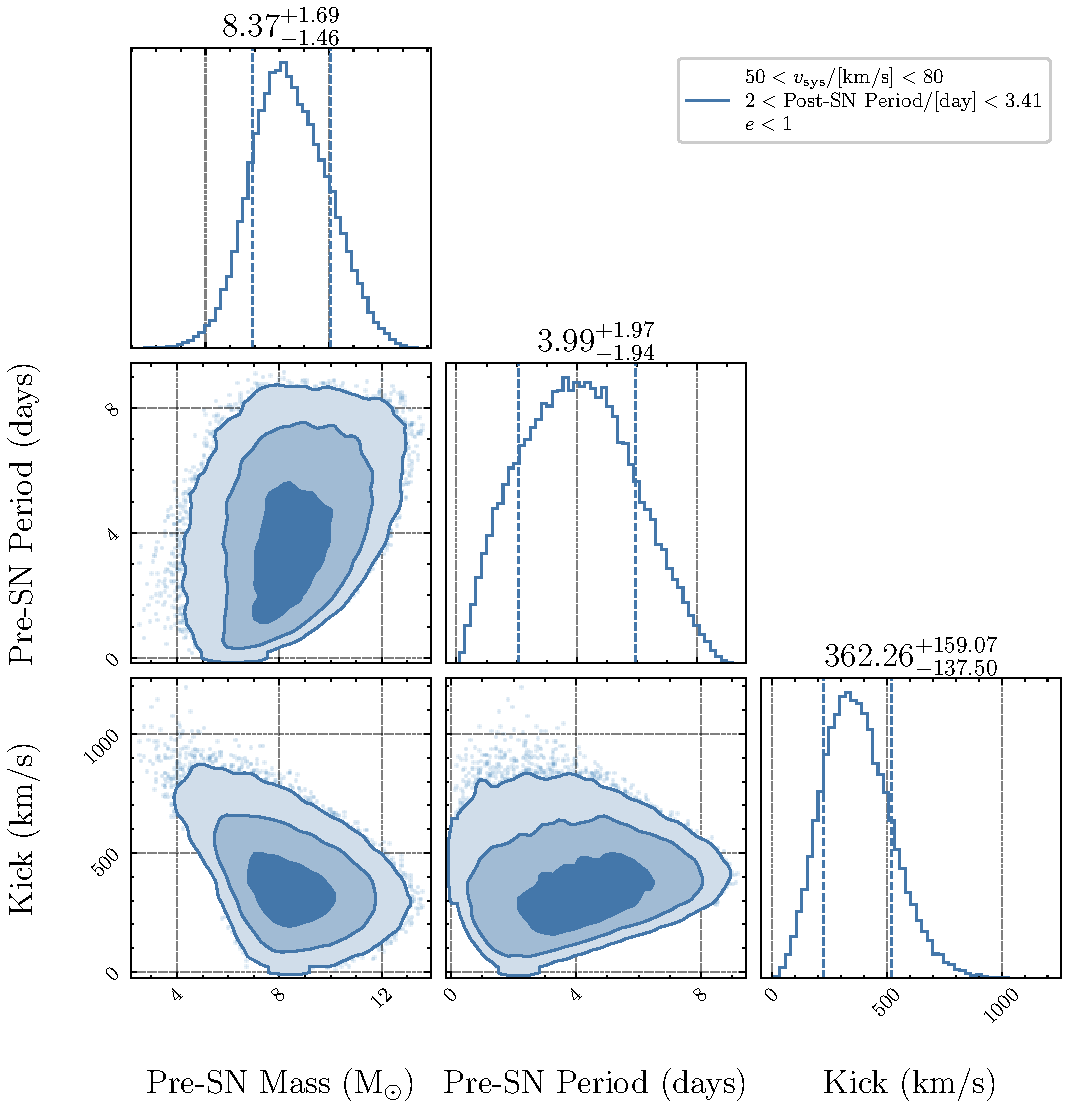
\includegraphics[width=0.5\textwidth]{xrb-monte-carlo-mass-period-kick.pdf}
    \caption{This is a caption for your figure.}
    \label{fig:xrb_monte_carlo}
\end{figure}

\subsection{Monte Carlo Results}

In this section, we describe the outcomes of our monte carlo simulations that simulate the effects of a supernova in a binary. Note that these are different from population synthesis simulations, as the initial binary population that we use is not observationally motivated, but is meant to explore the parameter space of interest relevant to the properties of the XRB. 

We start with generating $10^7$ binaries, with the following properties
 
\begin{enumerate}
        \item The mass of the companion star is uniformly sampled between $40-60M_{\odot}$. This roughly spans the measured mass of the visible star today, and we do not expect it to change significantly during the supernova and until today. In our simulations, we assume this mass to be fixed before and after the SN.
        \item For the progenitor of the $2.5M_{\odot}$ compact object, we sample the mass lost in the supernova explosion ($\Delta m$) uniformly between $0-20M_{\odot}$. We fix the post--SN mass of the compact object to be $2.5M_{\odot}$. The mass of the pre--SN star is then given by $2.5M_{\odot}+\Delta m$.
        \item We sample the pre--SN period of the binary uniformly between $0-30$ days.
        \item We sample the kick distribution from a maxwellian distribution with a scale of $265 km/s$ and isotropic in direction.
        \item We assume the pre-SN orbits to be circular.
\end{enumerate}

Now that we have defined our pre--SN population, we simulate the outcomes of a SN explosion on the properties of the binary. Depending on the amount of mass lost in the explosion and the strength and direction of the natal kick to the compact object, the orbit of the binary can change or it may even become unbound. It may also induce some eccentricity in the orbit, and give the center of mass of the binary a systemic velocity. By sampling different combinations of mass loss and kick vectors, we can infer which binaries get unbound, which ones are bound, and what are the new orbits of the bound systems. We then compare them to the observational constraints that we have for the XRB, and select for systems that satisfy those conditions.

The observational constraints that we impose are as follows 

\begin{enumerate}
        \item The orbital period post--SN is between $2-3.41$ days. We place a lower limit of 2 days as orbital periods smaller than this imply that the current visible star would have filled its roche lobe post--SN which does not seem plausible given its current evolutionary state. As the current orbital period is measured to be around $3.41$ days, we allow for post--SN periods smaller than this because wind mass loss post--SN could have widened the system to its current orbital period as well.
        \item The systemic velocity inherited during the SN is 50-80km/s (the measured systemic velocity with respect to the open cluster is ~65km/s). Here, we are making the assumption that most of the systemic velocity of the XRB with respect to its birth cluster today can be attributed to its post--SN systemic velocity. We are also implicitly assuming that this velocity has not significantly changed during its runaway phase for the past couple of Myr. However, the details of this would depend on accurately modeling the effects of the cluster potential, which we do not model in this work.
        \item We assume that the induced eccentricity in the binary is less than one, meaning that we only select for systems that remain bound post--SN (there are disagreements in literature on whether the binary is close to circular or has a modest eccentricity of ~0.2). Since the binary could have had a higher eccentricity post--SN (but less than one) and has undergone tidal circularization since then during the runaway phase, we do not impose any constraints based on its measured eccentricity (controversial) today.
\end{enumerate}

Fig. \ref{fig:xrb_monte_carlo} shows the distribution of binary parameters that satisfy the observational constraints of the XRB. We emphasize that the probability distributions here are not to be taken literally, as the probability distribution of the pre--SN population was not physically motivated. We find that the pre--SN mass of the progenitor of the compact object must have between $4-12M_{\odot}$. We also find that the pre--SN orbital period was likely smaller than $9$ days. Although we do not put any constraints on the pre--SN orbital period, it is likely that it could not have been very small ($<1-2$ days) as that would imply that the companion star would fill its roche lobe before the SN. We now point out some interesting regions in the corner plot that provide clues on the XRB's past. We find that large pre--SN periods ($>4$ days) and small or no kicks are incompatible, as it would not be possible to shrink the binary orbit to its post--SN period in such cases. This is important because mass transfer in binaries tends to widen th orbital period in most scenarios. Given that this XRB likely went through a phase of mass transfer in the past (from the progenitor of the CO onto the current visible star), its post--SN period was likely large enough that a natal kick is necessarily needed to shrink the orbit post--SN to its current state. 

Another excluded region in this plot is the lower left corner in the pre--SN period vs kick panel. This shows that small enough pre--SN periods and low kicks are incompatible with the imposed observational constraints. The reasons for this are a bit subtle, and we explain it for the case of no kicks, which can then be easily generalized to the presence of kicks. We have imposed a constraint that the post--SN period is larger than $2$ days, and the systemic velocity is smaller than $80\rm km/s$. For a small enough pre--SN period, it so happens that to widen the orbit to satisfy the imposed constraints, the systemic velocity required exceeds the observational constraints. However, kicks allow some room for scatter in such situations, and thus the minimum pre--SN period decreases as we increase the strength of the kicks, which creates the diagonal boundary in the lower left corner in the pre--SN period vs kick panel.

\subsection{Why do we need a natal kick?}

Compact object that are formed in a successful supernova explosion may receive a natal kick at birth due to asymmetries in the explosion or in neutrino emission. Observationally, the natal kicks received by neutron stars is well described by a maxwellian distribution with a mean of 265km/s. However, for black holes, the story is a bit more complicated with evidence pointing towards weak or no kicks in some cases or strong kicks in others. For our X-ray binary of interest, we know that this is a runaway system from Gaia kinematics. The runaway nature does not necessarily imply that the compact object received a natal kick, as some mass lost in a spherically symmetric can also impart a systemic velocity to the binary and also induce eccentricity in the system. This is referred to as the "Blauuw kick" and the new binary orbit (if the system did not get disrupted) always has a larger orbital period (and therefore the orbital separation) because of the mass lost in the explosion. However, a decrease in the orbital period may be possible given a natal kick in a favourable direction. Given that the XRB currently is in a very tight orbit of just 3.41 days, a Blauuw kick implies that the pre-supernova orbit must have been even tighter. This may be inconsistent with most scenarios of mass transfer through RLOF, which in general leads to a widening of the orbit. Therefore, we assume that the pre-supernova orbital period was larger than the current one, and that the shrinking of the orbit is due to a natal kick received by the compact object. Not just that, for the orbit to shrink, we find that the natal kick must be directed away from the orbital velocity of the star, as seen in (insert fig)

\section{Why not a common envelope?}

Given the short period of the XRB, it may seem appealing to invoke a common envelope formation scenario for this system. In this section, we discuss why it is difficult to form this X-ray binary through a common envelope instead of stable RLOF. To start with, the visible star in the system (and the originally less massive one) has a high mass of 40-60Msun. Since this star likely did not gain any mass during a supposed common envelope phase, the original donor that formed the compact object must have been more massive than 40-60 Msun. In a common envelope phase, the donor would lose its envelope, and leave behind a core that would be far too massive to successfully explode and form a 2.5Msun compact object (however see Burrows et al etc papers). To add to that, our monte carlo experiments imply that the pre-SN donor mass is less than 15Msun, which is far too small of a core for a star that is more massive than 40-60Msun. Also, common envelope phases usually are though to occur for asymmetric binaries, and this may imply that the donor should have been much more massive than the current visible star. All of these constraints may imply that forming this X-ray binary through a common envelope phase is unlikely, and that the likely scenario may involve stable mass transfer through RLOF.

\section{Why not Case B mass transfer?}

Previous studies of this system have suggested formation pathways wherein mass transfer occurs after the donor star has left the main sequence (Case B). However, this is unlikely because of the short orbital period of the binary today. Renzo 2019 (insert citation) showed that for Case B mass transfer, the orbital period of the binary widens significantly in most cases, except for scenarios where mass transfer is non conservative ($\beta < 0.6$) \textit{and} there are extreme losses in angular momentum ($\gamma_{\rm RLOF} \geq 2$). Even with a favourable kick in the right direction, it is likely extremely rare to get the period post core-collapse to less than 4 days.

\section{XRB}

HD153919 is a well studied runaway high mass X-ray binary. It consists of a bright O-type star with a compact companion that straddles the mass gap between the heaviest neutron stars and lightest black holes at 2.5Msun. The extreme mass ratio (~20 to 1), short orbital period and the runaway nature of the binary have been particularly challenging to simultaneously explain through standard formation channels. Using Hipparcos, and more recently with Gaia DR3, the binary can be confidently traced back to have originated from the young open cluster NGC6231. By measuring the systemic velocity with respect to the cluster, we know that the binary must have been kicked out ~2.2Myr ago. We also know that the cluster is very young with quite a few massive stars still present, with age estimates ranging from 4-10Myr. It is likely that a supernova explosion in the binary which formed the 2.5Msun compact object gave the system a systemic velocity that ejected it out of the cluster. Given the young age of the cluster at the time of explosion, the progenitor star that exploded must have originally been quite massive as well. Since this XRb is well studied, we have strong constraints on the binary's orbit, the individual masses and on the systemic velocity which presumably is dominated by the kick it received due to the supernova explosion. Given these constraints, we perform monte-carlo simulations to estimate what range of pre-supernova orbital configurations can explain the current observational constraints of the binary. We model the supernova explosion as an instantaneous mass loss event, and together with conservation of momentum, we can recompute the induced eccentricity in the binary. An eccentricity greater than one implies that the explosion disrupts the binary, while for eccentricities less than one we can recompute the new orbital period and separation, along with the systemic velocity induced in the binary due to the explosion. We also account for the effect of natal kicks that the compact object can receive during a supernova and its effect on the fate of the binary. To summarise, the observational constraints that we impose are

\subsection{Results -- XRB}

In this section, we describe the evolution of our supposed progenitor system of the HMXB 4U-1700-27. Motivated by the results of our monte carlo simulations, we start with a binary of initially masses $40M_{\odot}$ and $33.5M_{\odot}$ in a tight orbit with a period of just 3.5d. As a result, the donor overflows its roche lobe just after $3.48 \rm Myr$, during the Main Sequence (MS) itself. This leads to a phase of mass transfer from the donor to the accretor, commonly referred to as Case A. This phase actually consists of an initial thermal timescale mass transfer ($0.07\rm Myr$), known as fast Case A, where the donor loses a majority of the mass lost during RLOF. As the donor regains thermal equilibrium, it slowly grows in size on a nuclear timescale, which leads to a steady period of mass transfer referred to as slow Case A. This phase ends around $4.9\rm Myr$, roughly when the donor has finished its supply of hydrogen in its core, and it starts contracting on a thermal timescale, ending the first phase of RLOF. At this stage, the donor has lost around $15M_{\odot}$, with $11M_{\odot}$ lost during the thermal timescale fast Case A itself. It now has a mass of $24.7M_{\odot}$, and having lost much of its envelope, the surface now exposes the products of CNO--burning. It has a helium rich ($Y = 0.59$) and hot surface ($T_{\rm eff} \approx 37000K$), and a thin envelope of $\approx 6.8M_{\odot}$. Note that the mass of the helium core at this point is almost $18M_{\odot}$, which is potentially far too large to lead to a successful explosion. On the other hand, the accretor (still on the MS) has grown from its initial $33.5M_{\odot}$ to $\approx 45.5M_{\odot}$. Due to the increase in mass, it is now overluminous with a $\rm log_{10} (L/L_{\odot}) \approx 5.7$ and a surface temperature of $37000K$.

Case AB 

As the donor star still has a substantial amount of hydrogen left in its envelope, it ignites hydrogen burning in a shell, which drives a radid increase in its radius on a thermal timescale. As the binary only expanded from an initial period of $3.5d$ to $4.6d$, the donor star once again overflows its roche lobe during the hydrogen shell burning phase. As this occurs after the initial Case A mass transfer, this period is referred to as Case AB mass transfer (with the B referencing mass transfer occuring after the MS but before helium depletion). This also occurs on a thermal timescale, where the donor loses an additional $4M_{\odot}$, bringing its mass down to $19.4M_{\odot}$. Due to rotational spin down by tides, the accretor is able to accrete most of this mass, and it grows to almost $49.2M_{\odot}$. This phase ends just after $10000 \rm yr$ (when it happens is messy).  Since the donor is now even more stripped of hydrogen (surface $X \approx 0.2$), it starts contracting and has a higher surface temperature. It soon ignites helium in its center, and initiates the core helium burning phase, which lasts for $\approx 0.44 \rm Myr$. During this phase, it has a hot helium rich surface, and would resemble a Wolf--Rayet (WR) star with a strong optically thick wind. These mass loss rates are of the order of $10^{-5} - 10^{-6} M_{\odot}/\rm yr$, and the donor star loses an additional $11M_{\odot}$ during its WR phase until helium depletion. At this point we terminate our MESA models, and the originally more massive star now has a mass of $13.3M_{\odot}$, with a CO core mass of $11.3M_{\odot}$ (central $\rm C/O \approx 0.37$). There is no hydrogen left on the surface which is now mostly consisting of helium, carbon and some oxygen. Meanwhile, the originally less massive star (and the current visible/donor in the XRB) now has a mass of $48.2M_{\odot}$. The orbital period of the binary has now increased to $8.27d$, which aligns with the expectations from our monte carlo simulations.

Our monte-carlo simulations imply that the progenitor star of the compact object must have been ~7-14Msun prior to explosion. This is a strong indicator for past binary interaction, as the progenitor must have been much more massive early on given the young age of the cluster (atleast >30Msun). We also know that the companion is quite massive today, and this could be due to accretion of mass from the donor. These constraints hint towards an episode of stable and conservative mass transfer in the past, and our goal is to chart an evolutionary pathway from a pair of progenitor stars to the current observed X-ray binary. Motivated by the constraints from our monte-carlo sims, we model the evolution of a binary consisting of 2 massive star of 40 and 30Msun in a short orbit of 4 days. At such short periods, tides efficiently circularize and synchronize the orbit. Due to the small separation between the stars, the more massive star overflows its roche lobe during its Main Sequence itself, starting a phase of mass transfer that is commonly referred to as Case A mass transfer. 

\begin{figure}[htbp]
    \centering
    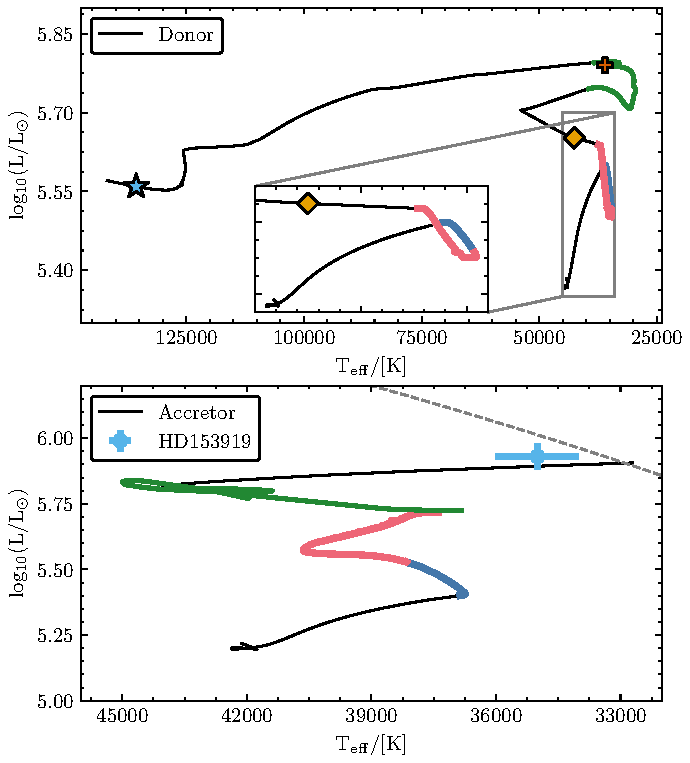
\includegraphics[width=0.5\textwidth]{xrb_fiducial_hr.pdf}
    \caption{This is a caption for your figure.}
    \label{fig:xrb_fiducial_hr}
\end{figure}

\section{GW190814}

GW190814 was an exceptional event that consisted of a merger between a 23Msun black hole and 2.5Msun compact object. The GW data alone was not enough to characterize the black hole or neutron star nature of the less massive compact object, and the formation of such a system of such an asymmetric mass ratio has been puzzling for standard formation channels. 

\section{Future evolution}

Now that we have been able to chart a reasonable past evolutionary history of the XRB using our MESA binary models, we evolve the system further to see what the future of this system could look like? The current mass of the compact object is 2.5Msun while the companion is 40-60Msun that is yet to fill its roche lobe. As the star evolves further, it will grow in size and soon overflow its roche lobe. However, given the highly asymmetric nature of the system, the subsequent mass transfer is likely to soon become unstable and the compact object will plunge into the companion star's envelope, starting a phase of common envelope evolution. This phase is highly complex and multidimensional with various physical processes occuring at different time and length scales. Importantly, the success or failure of the common envelope phase is an active area of research with no concrete predictions. However, various techniques have been introduced to simulate (or skip over) this phase, enabling predictions to be made albeit at the cost of accuracy. One of the most commonly used approaches is the energy balance formalism or $\alpha \lambda$ mechanism. This parameterized method quantifies what fraction ($\alpha$) of the orbital energy is required to unbind the donor star's envelope, which is parametrized by $\lambda$. To simulate the outcome of our XRB, we evolve it till it overflows its roche lobe and the mass transfer becomes unstable (quantified by Mdot > 0.1Msun/yr). Using the orbital separation, we know how much orbital energy is available, and using the interior structure of the star, we can compute the binding energy of the envelope as well. This requires us to assume a particular definition of core, and everything above it would be considered the envelope. If a common envelope ejection is successful, what remains of the donor star is its core, and we assume that it may have some sort of response that can expand its size by up to twice that of what the core size originally was at the star of the common envelope phase. If we assume a perfect use of orbital energy to unbind the envelope, i.e $\alpha=1$, we can compute what would be the final separation between the compact object and the remnant core. If the remnant core fits inside the roche lobe of its new orbit, it implies that common envelope ejection was successful and we are left with a tight but detached binary. However, if the remnant core is too large for its final orbit, it means that there was a merger between the compact object and remnant core, and common envelope ejection was not successful. 




\section{Results} \label{sec:floats}
\begin{itemize}
    \item constrain pre-SN of XRB with monte carlo
    \item past evolutionary history with Zsolar MESA models
    \item future of XRB (TZO?)
    \item
    \item
    \item
    \item
    \item
    \item
\end{itemize}
% > constrain pre-SN of XRB with monte carlo
% > past evolutionary history with Zsolar MESA models
% > future of XRB
% 	> TZO?
% > figures
% 	> pre-SN constraints of XRB via monte carlo
% 	> mesa models on HR diagram
% 	> evolution of properties over time (mass, separation, etc)
% 	> future of XRB? failed CE (binding energy etc)

\section{Discussion} \label{sec:highlight}

\section{Conclusion} \label{sec:cite}


%% Please use the acknowledgment and contribution environments. This will 
%% be anonomyized when the "anonymous" style option is used. 
\begin{acknowledgments}

\end{acknowledgments}

\begin{contribution}

\end{contribution}

%% To help institutions obtain information on the effectiveness of their 
%% telescopes the AAS Journals has created a group of keywords for telescope 
%% facilities.
%
%% Following the acknowledgments section, use the following syntax and the
%% \facility{} or \facilities{} macros to list the keywords of facilities used 
%% in the research for the paper.  Each keyword is check against the master 
%% list during copy editing.  Individual instruments can be provided in 
%% parentheses, after the keyword, but they are not verified.
\facilities{HST(STIS), Swift(XRT and UVOT), AAVSO, CTIO:1.3m, CTIO:1.5m, CXO}

%% Similar to \facility{}, there is the optional \software command to allow 
%% authors a place to specify which programs were used during the creation of 
%% the manuscript. Authors should list each code and include either a
%% citation or url to the code inside ()s when available.
\software{astropy \citep{2013A&A...558A..33A,2018AJ....156..123A,2022ApJ...935..167A},  
          Cloudy \citep{2013RMxAA..49..137F}, 
          Source Extractor \citep{1996A&AS..117..393B}
          }

%% Appendix material should be preceded with a single \appendix command.
%% There should be a \section command for each appendix. Mark appendix
%% subsections with the same markup you use in the main body of the paper.
%%
%% Each Appendix (indicated with \section) will be lettered A, B, C, etc.
%% The equation counter will reset when it encounters the \appendix
%% command and will number appendix equations (A1), (A2), etc. The
%% Figure and Table counter will not reset.

\appendix

%% For this sample we use BibTeX plus aasjournalv7.bst to generate the
%% the bibliography. The sample7.bib file was populated from ADS. To
%% get the citations to show in the compiled file do the following:
%%
%% pdflatex sample7.tex
%% bibtext sample7
%% pdflatex sample7.tex
%% pdflatex sample7.tex

\bibliography{xrb_gw}{}
\bibliographystyle{aasjournalv7}

%% This command is needed to show the entire author+affiliation list when
%% the collaboration and author truncation commands are used.  It has to
%% go at the end of the manuscript.
%\allauthors

%% Include this line if you are using the \added, \replaced, \deleted
%% commands to see a summary list of all changes at the end of the article.
%\listofchanges

\end{document}

% End of file `sample7.tex'.
